\documentclass[a4paper,11pt]{report}
\usepackage{fullpage}

\usepackage{"../../info/packages"}
\usepackage{"../../info/nomenclature"}

\usepackage{scalerel}
\usepackage{subfiles}

\newcommand{\xvecdot}{\dot{\xvec}}
\newcommand{\xdot}{\dot{x}}
\newcommand{\qvecdot}{\dot{\qvec}}
\newcommand{\qdot}{\dot{q}}

\setlength{\cellspacetoplimit}{3pt}
\setlength{\cellspacebottomlimit}{3pt}

\title{Laser-plasma interactions}
\author{Alejandro Campos}

\begin{document}
\maketitle
\tableofcontents

%########################################################################
\chapter{Some notes on lasers}
%########################################################################
Consider a wave that depends on time $t$ and single spatial dimension $x$, which is orthogonal to the direction of propagation. 

A wave is spatially coherent at a given time $t$, position $x$, and separation distance $L$ if the phase difference between the points $x$ and $x+L$ at time $t$ is the same as that at a later time $t+dt$. You can keep on picking larger and larger values of $L$ until this is not the case, this $L$ would be the spatial coherence length $L_c$ = $L_c(t,x)$.

A wave is temporally coherent at a given time $t$, position $x$, and separation time $\tau$ if the phase difference between times $t$ and $t+\tau$ at position $x$ is the same as that between times $t+dt$ and $t+dt+\tau$. You can keep on picking larger and larger values of $\tau$ until this is no longer the case, this $\tau$ would be the temporal coherence length $\tau_c = \tau_c(t,x)$.

\begin{figure}
    \centering
    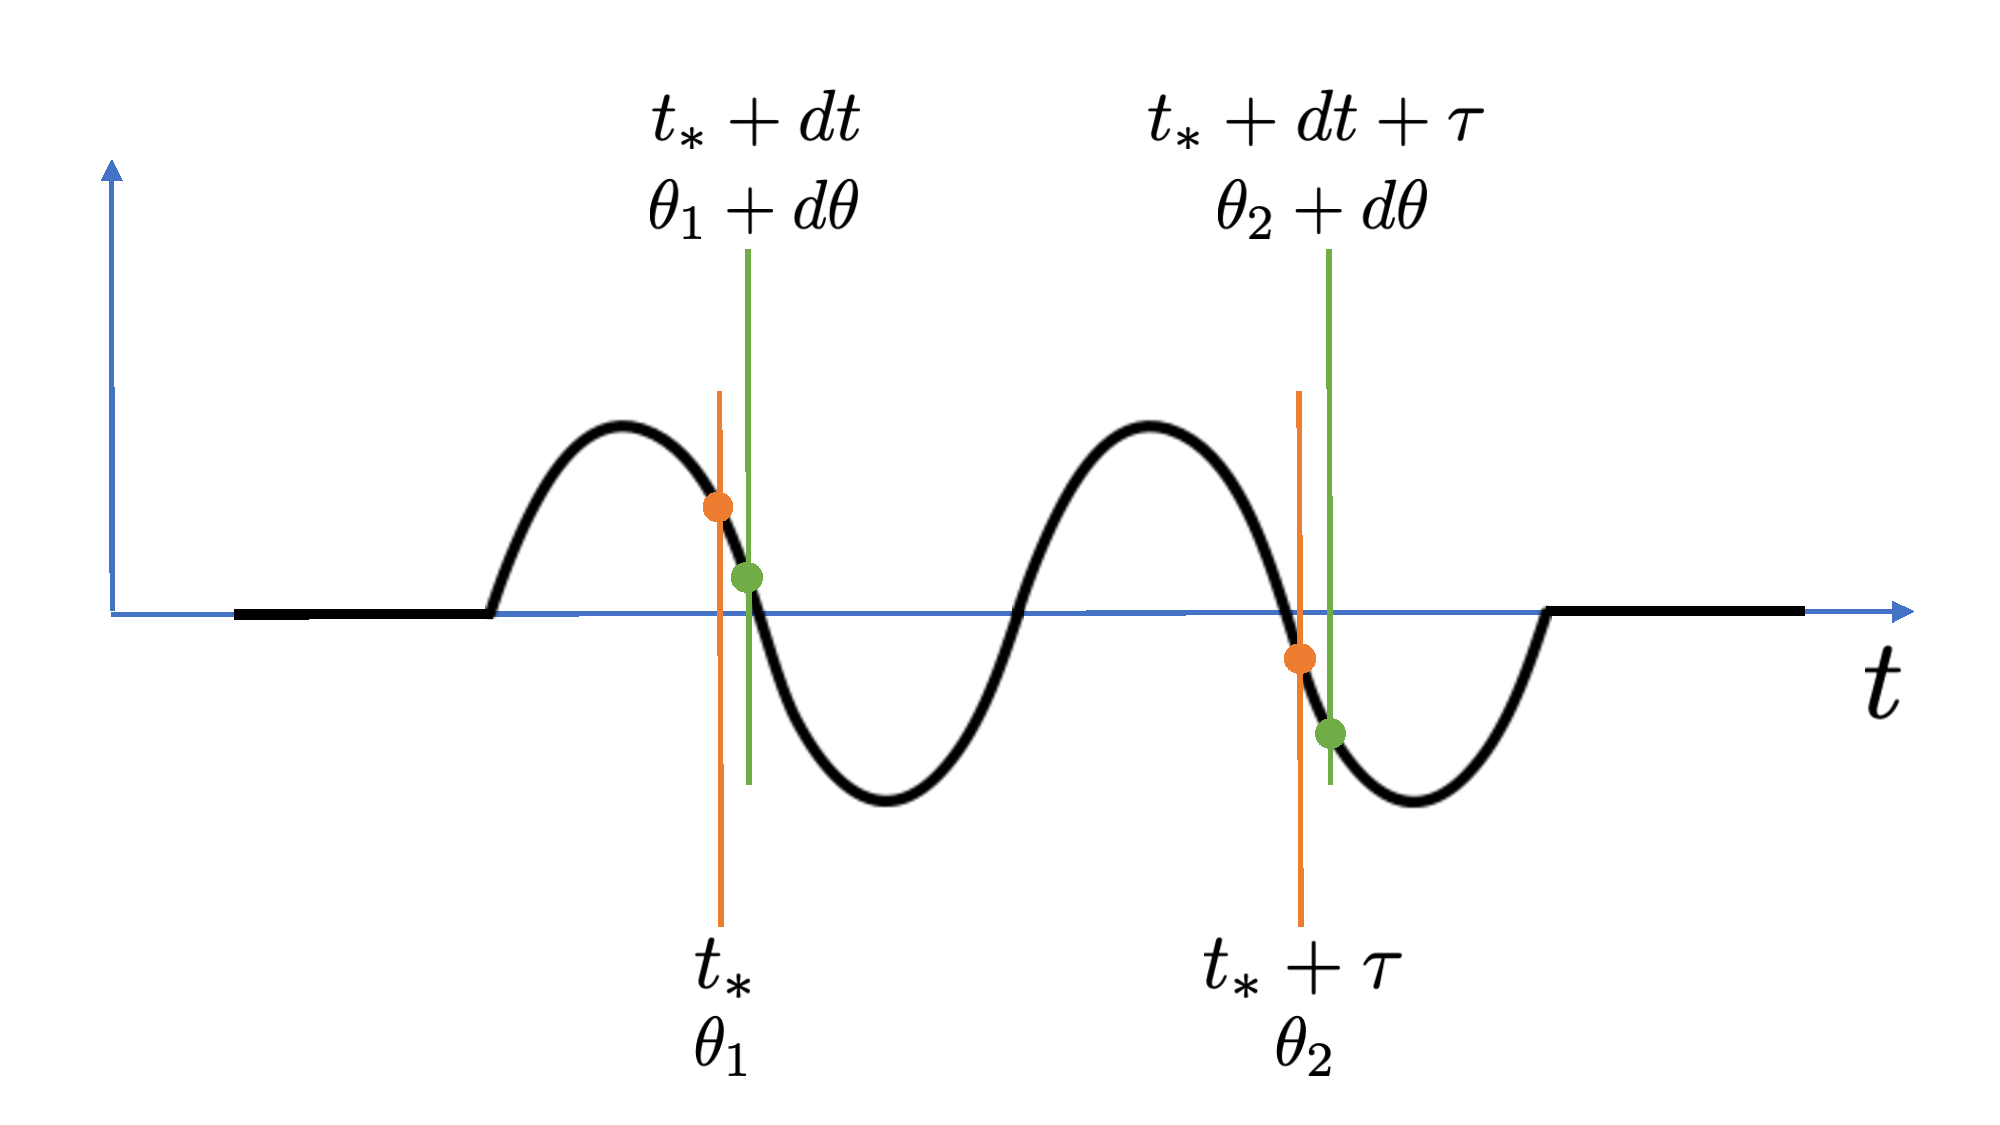
\includegraphics[width=.7\textwidth]{../../images/temp_cohe_1.pdf}
    \caption{}
    \label{fig:laser_temp_cohe}
\end{figure}

\begin{figure}
    \centering
    \begin{subfigure}{.7\textwidth}
      \centering
      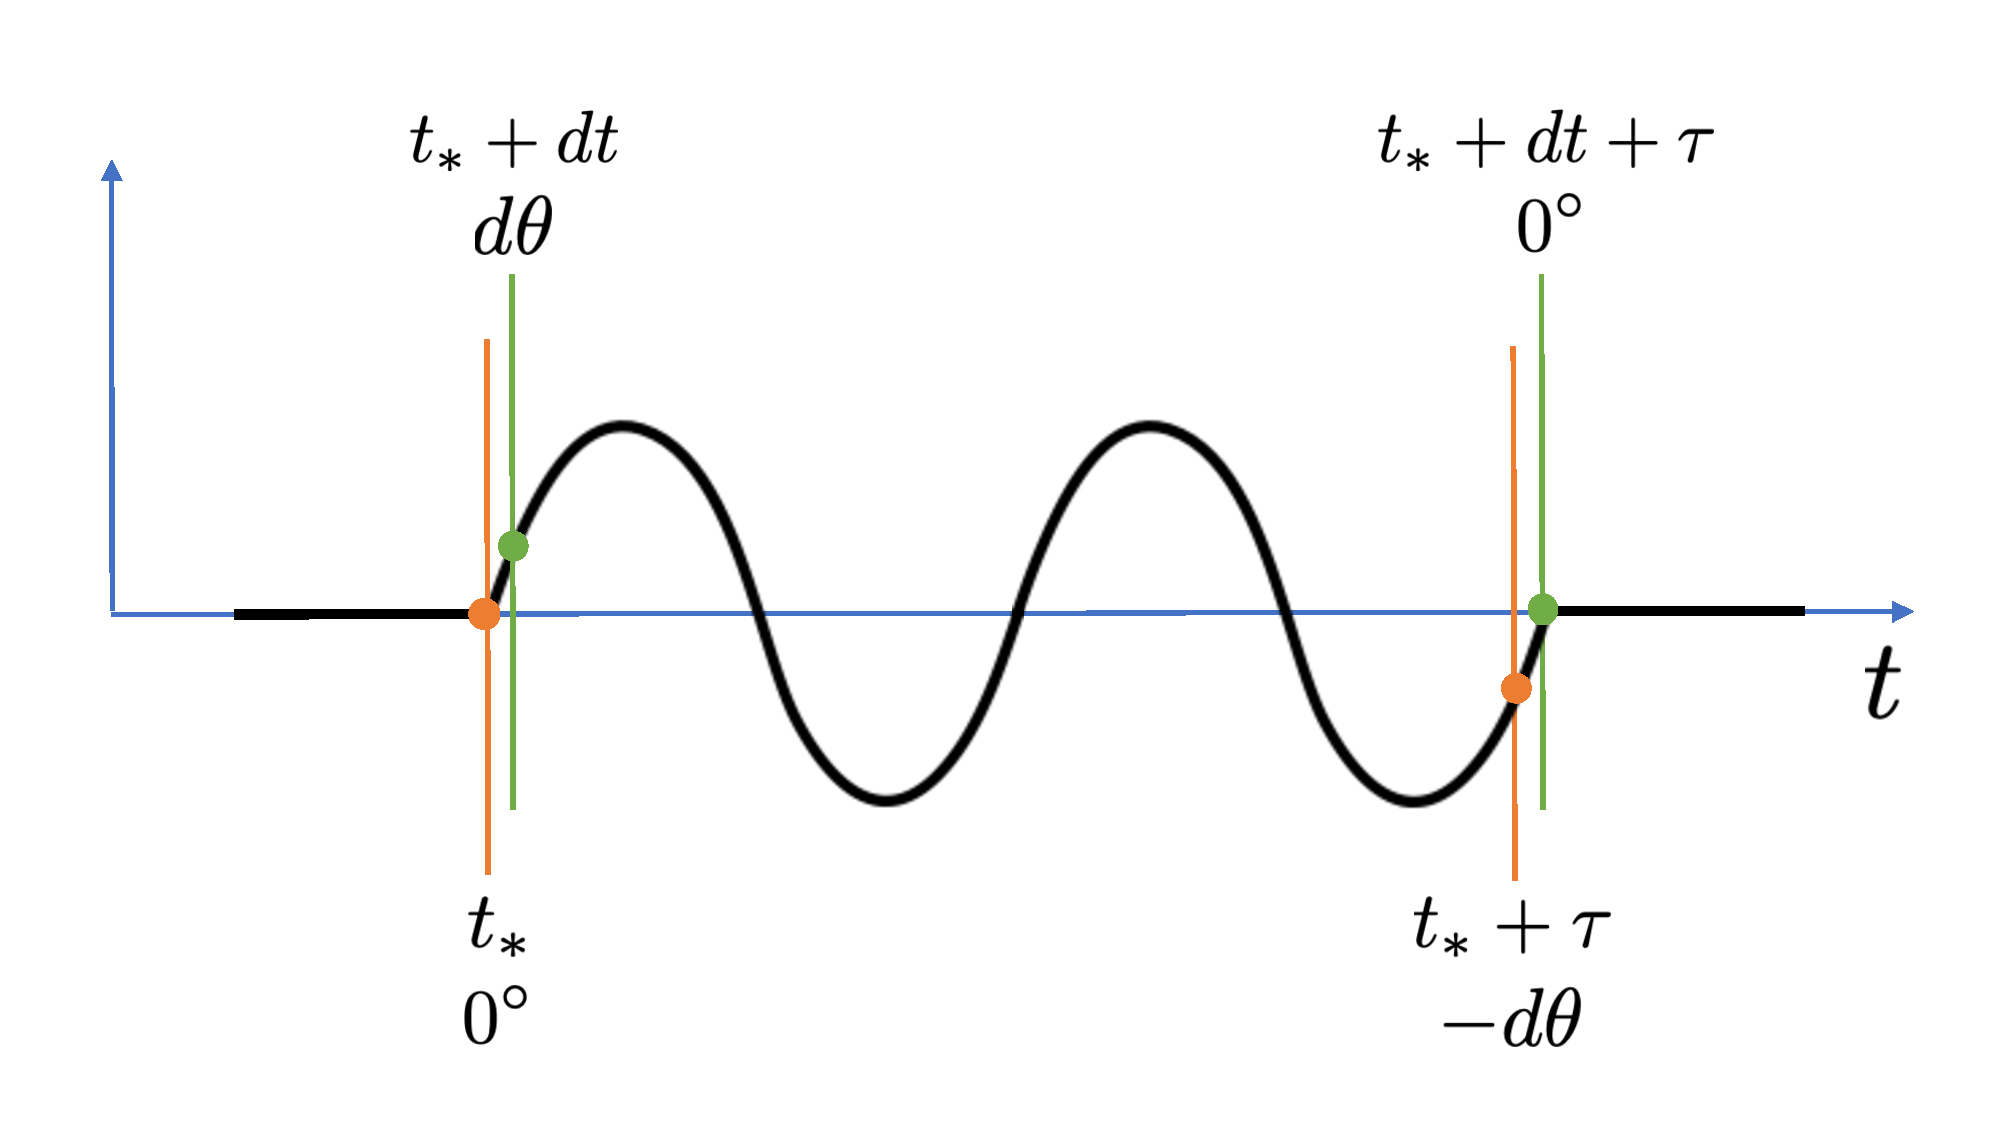
\includegraphics[width=\textwidth]{../../images/temp_cohe_2.pdf}
      \caption{}
      \label{fig:laser_temp_cohe_1}
    \end{subfigure}
    \begin{subfigure}{.7\textwidth}
        \centering
        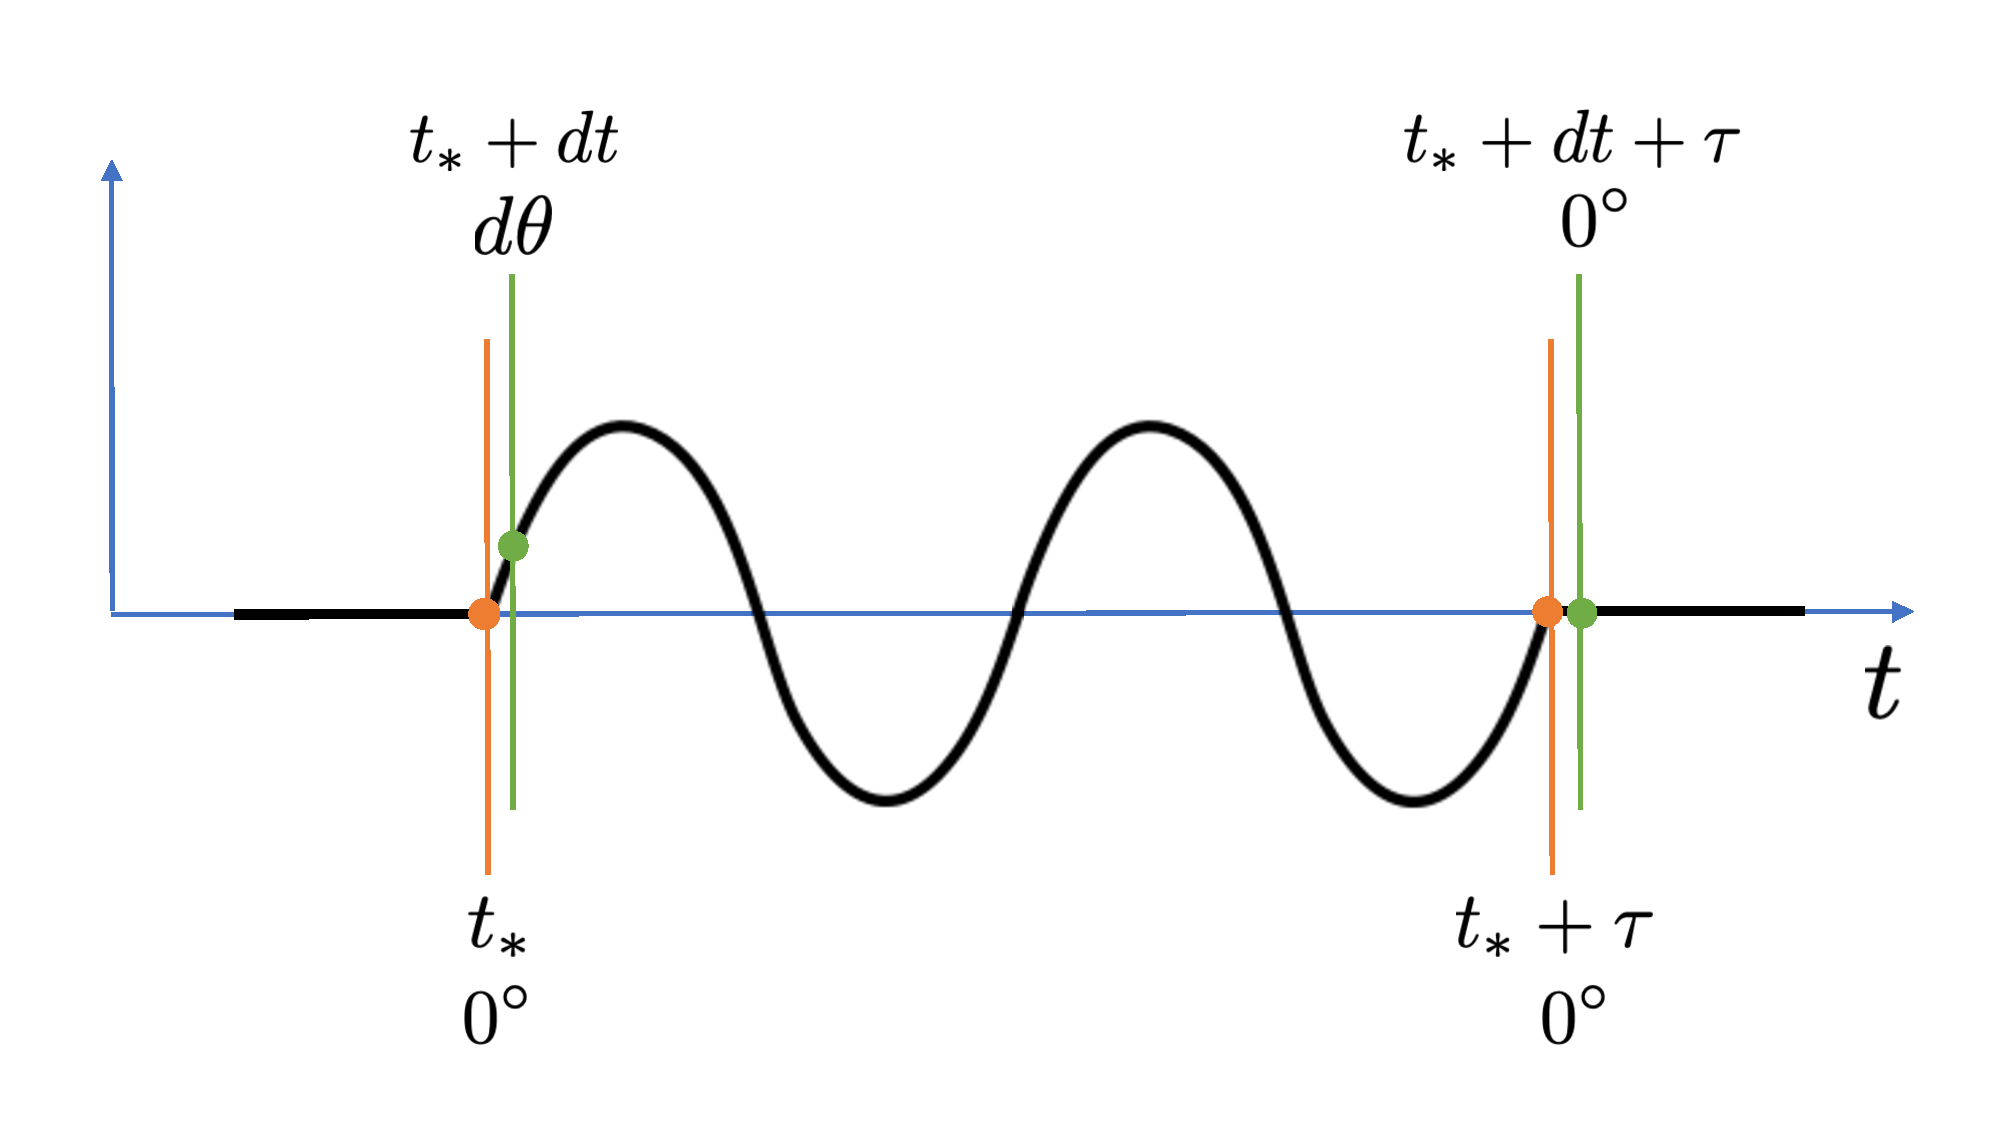
\includegraphics[width=\textwidth]{../../images/temp_cohe_3.pdf}
        \caption{}
        \label{fig:laser_temp_cohe_2}
      \end{subfigure}
    \caption{Depiction of temporal coherence for a light pulse.}
    \label{fig:laser_temp_cohe_12}
\end{figure}

A depiction of temporal coherence is provided in \cref{fig:laser_temp_cohe}, which shows a light pulse as a function of time. An arbitrary time $t_*$ is chosen along the light wave, and the wave's phase at that time is $\theta_1$. At the time $t_* + \tau$ the wave has a different phase $\theta_2$, and thus the phase difference between times $t_*$ and $t_*+\tau$ is $\theta_2 - \theta_1$. This is depicted by the orange dots. The green dots are used to highlight the phase difference between times $t_*+dt$ and $t_*+dt+\tau$. In this case, the phases are respectively $\theta_1 + d\theta$ and $\theta_2 + d\theta$, and hence the phase difference is still maintained at $\theta_2 - \theta_1$.

Rather than picking the time $t_*$ to be at an arbitrary location along the wave, in \cref{fig:laser_temp_cohe_1} we choose $t_*$ to be at the beginning of the wave, and also choose $\tau$ to be just a bit smaller than the entire duration of the pulse. For this case, the phase difference between $t_*$ and $t_*+\tau$ is $d\theta$, which is equal to the phase difference between $t_*+dt$ and $t_*+dt+\tau$. On the other hand, in \cref{fig:laser_temp_cohe_2} we have chosen $\tau$ to be just a bit larger so as to be equal to the duration of the wave. For this case the phase difference between $t_*$ and $t_*+\tau$ is zero, which is not the same as the phase difference between $t_*+dt$ and $t_*+dt+\tau$, namely $d\theta$. Thus, the maximum value of $\tau$ that maintains a constant phase difference has been reached, and therefore by definition this value is referred to as the temporal coherence length $\tau_c$ at time $t_*$ (other locations of $t_*$, such as that in \cref{fig:laser_temp_cohe}, have a different $\tau_c$).

%########################################################################
\chapter{The baseline plasma model}
%########################################################################
We rely on the single-material two-fluid model under homentropic assumptions, which is summarized below
\begin{equation}
    \label{eq:pwaves_ion_density}
    \frac{\partial n_i}{\partial t} + \nabla \cdot \left (n_i \uvec_i \right ) = 0,
\end{equation}
\begin{equation}
    \label{eq:pwaves_electron_density}
    \frac{\partial n_e}{\partial t} + \nabla \cdot \left (n_e \uvec_e \right ) = 0,
\end{equation}
\begin{equation}
    \label{eq:pwaves_ion_momentum}
    \frac{\partial m_i n_i \uvec_i}{\partial t} + \nabla \cdot \left ( m_i n_i \uvec_i \uvec_i \right ) - Ze n_i \left ( \Evec + \uvec_i \times \Bvec \right ) = -\nabla p_i,
\end{equation}
\begin{equation}
    \label{eq:pwaves_electron_momentum}
    \frac{\partial m_e n_e \uvec_e}{\partial t} + \nabla \cdot \left ( m_e n_e \uvec_e \uvec_e \right ) + e n_e \left ( \Evec + \uvec_e \times \Bvec \right ) = -\nabla p_e,
\end{equation}
\begin{equation}
    \label{eq:pwaves_ion_pressure}
    p_i = C_i n_i^{\gamma_i},
\end{equation}
\begin{equation}
    \label{eq:pwaves_electron_pressure}
    p_e = C_e n_e^{\gamma_e},
\end{equation}
\begin{equation}
    \label{eq:pwaves_maxwell_3}
    \nabla \cdot \Evec = \frac{\rho_q}{\epsilon_0},
\end{equation}
\begin{equation}
    \label{eq:p_waves_maxwell_4}
    \nabla \cdot \Bvec = 0,
\end{equation}
\begin{equation}
    \label{eq:p_waves_maxwell_1}
    \nabla \times \Evec = -\frac{ \partial \Bvec}{\partial t},
\end{equation}
\begin{equation}
    \label{eq:p_waves_maxwell_2}
    \nabla \times \Bvec = \mu_0 \Jvec + \mu_0 \epsilon_0 \frac{\partial \Evec}{\partial t},
\end{equation}
\begin{equation}
    \label{eq:p_waves_curr_density}
    \Jvec = e (Z n_i \uvec_i - n_e \uvec_e),
\end{equation}
\begin{equation}
    \label{eq:p_waves_mass_density}
    \rho_q = e (Z n_i - n_e),
\end{equation}
\begin{equation}
    p_i = n_i k_B T_i,
\end{equation}
\begin{equation}
    p_e = n_e k_B T_e.
\end{equation}

%########################################################################
\chapter{Longitudinal and transverse waves}
%########################################################################

%------------------------------------------------------------------------
\section{Definitions}
%------------------------------------------------------------------------
The Helmholtz decomposition for a function $\Fvec = \Fvec(\xvec,t)$ is of the following form
\begin{equation}
    \Fvec = \Fvec_l + \Fvec_t,
\end{equation}
where $\Fvec_l = \Fvec_l(\xvec,t)$ is the longitudinal component and $\Fvec_t = \Fvec_t(\xvec,t)$ the transverse component. These are defined by
\begin{align}
    \nabla \times \Fvec_l &= 0, \label{eq:ltw_plasma_long_def}\\
    \nabla \cdot \Fvec_t &= 0. \label{eq:ltw_plasma_tran_def}
\end{align}
We'll assume that any vector function $\Gvec = \Gvec(\xvec,t)$ can be expressed as the real component of
\begin{equation}
    \label{eq:em_more_general_wave_form}
    \Gvec = \hat{\Gvec} \exp \left [ i \left ( \int_0^x k_x(x') \, dx' + \int_0^y k_y(y') \, dy' + \int_0^z k_z(z') \, dz'  - wt \right ) \right ].
\end{equation}
For the above, $w$ a frequency constant in time and space, and $k_x = k_x(x)$, $k_y = k_y(y)$, and $k_z = k_z(z)$ form the wave vector $\kvec = [k_x, k_y, k_z]$. $\hat{\Gvec} = \hat{\Gvec}(\xvec,t)$ is a complex vector where the real and complex components point in the same direction. Additionally, we enforce the constraint that if $\nabla \times \Gvec = 0$, then $\nabla \times \hat{\Gvec} = 0$, and similarly, if $\nabla \cdot \Gvec = 0$, then $\nabla \cdot \hat{\Gvec} = 0$. We'll often use a different subscript in the wave vectors and frequencies of different waves. For example, we'll use $\kvec_e$ for electron-plasma waves, $\kvec_i$ for ion-acoustic waves, $\kvec_L$ for laser waves, and $\kvec_s$ for scattered waves. Similarly for the frequencies $w_e$, $w_i$, $w_L$, $w_s$.

We note that
\begin{multline}
    \nabla \exp \left [ i \left ( \int_0^x k_x(x') \, dx' + \int_0^y k_y(y') \, dy' + \int_0^z k_z(z') \, dz'  - wt \right ) \right ] \\
    = i \kvec \exp \left [ i \left ( \int_0^x k_x(x') \, dx' + \int_0^y k_y(y') \, dy' + \int_0^z k_z(z') \, dz'  - wt \right ) \right ]
\end{multline}
Given the identity $\nabla \times (\Avec f) = (\nabla \times \Avec ) f - \Avec \times (\nabla f)$, we can show that
\begin{align}
    \label{eq:ltw_no_curl}
    \nabla \times \Gvec &= \nabla \times \left [ \hat{\Gvec} \exp (...) \right ] \nonumber \\
    &= \left ( \nabla \times \hat{\Gvec} \right ) \exp (...) - \hat{\Gvec} \times \left [ \nabla \exp (...) \right ] \nonumber \\
    &= \left ( \nabla \times \hat{\Gvec} \right ) \exp (...) - \hat{\Gvec} \times \left [ i\kvec \exp (...) \right ] \nonumber \\
    &= \left ( \nabla \times \hat{\Gvec} \right ) \exp (...) + i \kvec \times \Gvec.
\end{align}
Given the identity $\nabla \cdot (\Avec f) = ( \nabla \cdot \Avec) f + \Avec \cdot (\nabla f)$, we can show that
\begin{align}
    \label{eq:ltw_no_div}
    \nabla \cdot \Gvec &= \nabla \cdot \left [ \hat{\Gvec} \exp (...) \right ] \nonumber \\
    &= \left ( \nabla \cdot \hat{\Gvec} \right ) \exp (...) + \hat{\Gvec} \cdot \left [ \nabla \exp (...) \right ] \nonumber \\
    &= \left ( \nabla \cdot \hat{\Gvec} \right ) \exp (...) + \hat{\Gvec} \cdot \left [ i \kvec \exp (...) \right ] \nonumber \\
    &= \left ( \nabla \cdot \hat{\Gvec} \right ) \exp (...) + i \kvec \cdot \Gvec.
\end{align}
By definition, $\Fvec_l$ has no curl and $\Fvec_t$ has no divergence. As mentioned earlier, we then require $\hat{\Fvec}_l$ to have no curl and $\hat{\Fvec}_t$ to have no divergence. Using this in \cref{eq:ltw_no_curl,eq:ltw_no_div} allow us to write
\begin{align}
    \kvec \times \Fvec_l = 0 \label{eq:ltw_plasma_long_wavevector} \\
    \kvec \cdot \Fvec_t = 0 \label{eq:ltw_plasma_trans_wavevector}.
\end{align}

The first expression above says $\Fvec_l$ is parallel to $\kvec$ and the second says $\Fvec_t$ is orthogonal to $\kvec$. Thus, $\Fvec_l \cdot \Fvec_t = 0$. We will often have situations where $\nabla \times \Fvec = \nabla \cdot \Fvec = 0$, which by its own does not imply $\Fvec = 0$. However, using \cref{eq:ltw_no_curl,eq:ltw_no_div}, this translates to to $\kvec \times \Fvec = \kvec \cdot \Fvec =  0$. The latter equality states that $\kvec$ and $\Fvec$ are orthogonal, that is, the angle between them is $90^\circ$. The former equality leads to $|\Fvec| \sin(90^\circ) = 0$, which in turn means $\Fvec = 0$. To summarize,
\begin{equation}
    \label{eq:ltw_general_null_vector}
    \nabla \times \Fvec = \nabla \cdot \Fvec = 0 \to \Fvec = 0.
\end{equation}

For some cases we'll further restrict $\hat{\Gvec}$ in \cref{eq:em_more_general_wave_form} such that $\hat{\Gvec} = \hat{\Gvec} (\xvec)$, that is, the time dependence of the wave is fully captured by the $\exp(-iwt)$ term. For this case, we'll often re-write the expression for $\Gvec$ as
\begin{equation}
    \label{eq:em_semi_general_wave_form}
    \Gvec = \tilde{\Gvec} \exp (-iwt),
\end{equation}
where $\tilde{\Gvec} = \tilde{\Gvec}(\xvec)$ is given by
\begin{equation}
    \tilde{\Gvec} = \hat{\Gvec} \exp \left [ i \left ( \int_0^x k_x(x') \, dx' + \int_0^y k_y(y') \, dy' + \int_0^z k_z(z') \, dz' \right ) \right ].
\end{equation}
Finally, a further simplification occurs when $\kvec$ and $\hat{\Gvec}$ are assumed to be constant in space. For this case, the expression for $\Gvec$ becomes
\begin{equation}
    \label{eq:em_general_wave_form}
    \Gvec = \hat{\Gvec} \exp \left [i\left ( \kvec \cdot \xvec - wt \right ) \right ].
\end{equation}
These are the so-called plane waves. We end with the cautionary note that the second gradients of $\Gvec$ in \cref{eq:em_more_general_wave_form} are not necessarily the same as those of $\Gvec$ in \cref{eq:em_general_wave_form}.

%------------------------------------------------------------------------
\section{Electron-plasma and ion-acoustic waves}
%------------------------------------------------------------------------
For both electron-plasma and ion-acoustic waves we can assume the magnetic field does not change. Thus, Faraday's law gives
\begin{equation}
    \nabla \times \Evec = \nabla \times \Evec_t = 0.
\end{equation}
By definition, $\nabla \cdot \Evec_t = 0$. Thus, using \cref{eq:ltw_general_null_vector} we get $\Evec_t = 0$, that is, $\Evec = \Evec_l$. 

For electron-plasma waves, we have (see notes on electron-plasma waves)
\begin{equation}
    \label{eq:ep_waves_mom_linearized}
    \frac{\partial n_{e0} \uvec_{e1}}{\partial t} + \frac{e n_{e0}}{m_e} \Evec_1 = - \frac{\gamma_e k_B T_e}{m_e} \nabla n_{e1}.
\end{equation}
We can use \cref{eq:em_general_wave_form} to write the above in spectral form and thus obtain
\begin{equation}
-i w n_{e0} \hat{\uvec}_{e1} + \frac{e n_{e0}}{m_e} \hat{\Evec}_{1,l} = -\kvec_e \frac{\gamma_e p_{e0}}{n_{e0} m_e} \hat{n}_{e1}. 
\end{equation}
Since the second term on the left-hand side and the term on the right-hand side point along $\kvec_e$, $\hat{\uvec}_{e1}$ also points along $\kvec_e$, that is, $\hat{\uvec}_{e1} = \hat{\uvec}_{e1,l}$.

For ion-acoustic waves, we have (see notes on ion-acoustic waves)
\begin{equation}
    \label{eq:ia_waves_mom_linearized}
    \frac{\partial n_{i0} \uvec_{i1}}{\partial t} - \frac{Z e n_{i0}}{m_i} \Evec_1 = - \frac{\gamma_i k_B T_i}{m_i} \nabla n_{i1}.
\end{equation}
We can use \cref{eq:em_general_wave_form} to write the above in spectral form and thus obtain
\begin{equation}
-i w n_{i0} \hat{\uvec}_{i1} - \frac{Z e n_{i0}}{m_i} \hat{\Evec}_{1,l} = -\kvec_i \frac{\gamma_i p_{i0}}{n_{i0} m_i} \hat{n}_{i1}. 
\end{equation}
Since the second term on the left-hand side and the term on the right-hand side point along $\kvec_i$, $\hat{\uvec}_{i1}$ also points along $\kvec_i$, that is, $\hat{\uvec}_{i1} = \hat{\uvec}_{i1,l}$. Finally, we note that the electric field being purely longitudinal is in agreement with the linearized electron momentum equation, namely (see notes on ion acoustic waves)
\begin{equation}
    \label{eq:ia_waves_E}
    e n_{e0} \Evec_1 = -\gamma_e k_B T_e \nabla n_{e1}.
\end{equation}

%########################################################################
\chapter{Electromagnetic waves in plasmas}
%########################################################################

\label{sec:electromagnetic_waves_plasmas}
In introductory electrodynamics, one typically studies electromagnetic waves in vacuum, that is, for cases where $\rho_q = \Jvec = 0$. In this section we relax both of these assumptions. Consider the electric and magnetic fields as well as the scalar and vector potentials, which satisfy
\begin{equation}
    \label{eq:emp_general_E_potential}
    \Evec = -\nabla \phi - \frac{\partial \Avec}{\partial t},
\end{equation}
\begin{equation}
    \label{eq:emp_general_B_potential}
    \Bvec = \nabla \times \Avec.
\end{equation}
For the above, we choose $\nabla \cdot \Avec = 0$. Using the fact that the magnetic field is solenoidal, we have
\begin{equation*}
    \nabla \cdot \Bvec = \nabla \cdot \Bvec_l + \nabla \cdot \Bvec_t = \nabla \cdot \Bvec_l = 0.
\end{equation*}
However, by definition, $\nabla \times \Bvec_l = 0$ as well. Thus, using \cref{eq:ltw_general_null_vector}, we have $\Bvec_l = 0$. The same argument applies to the vector potential, and thus $\Avec_l = 0$. For the electric field, we have
\begin{equation*}
    \nabla \cdot \Evec = \nabla \cdot \Evec_l + \nabla \cdot \Evec_t = \nabla \cdot \Evec_l .
\end{equation*}
Taking the divergence of \cref{eq:emp_general_E_potential}, we get
\begin{equation}
    \nabla \cdot \Evec = \nabla \cdot \left ( -\nabla \phi \right ).
\end{equation}
Combining the last two equations gives
\begin{equation*}
    \nabla \cdot \left ( \Evec_l + \nabla \phi \right ) = 0.
\end{equation*}
By definition, we also have
\begin{equation*}
    \nabla \times \left ( \Evec_l + \nabla \phi \right ) = 0.
\end{equation*}
Thus, using \cref{eq:ltw_general_null_vector}, we have $\Evec_l = -\nabla \phi$. A similar argument can be used to show $\Evec_t = -\partial \Avec / \partial t$. Our goal in this section will be to determine equations for $\Evec_l$, $\Evec_t$ and $\Bvec$.

We'll begin with the conservation of charge equation
\begin{equation*}
    \frac{\partial \rho_q}{\partial t} + \nabla \cdot \Jvec = 0,
\end{equation*}
which we re-write as
\begin{equation*}
    \frac{\partial \rho_q}{\partial t} + \nabla \cdot \Jvec_l = 0,
\end{equation*}
Using Poisson's equation $\nabla^2\phi = -\rho_q / \epsilon_0$ in the above, we get
\begin{equation*}
    \frac{\partial}{\partial t} \left ( -\epsilon_0 \nabla^2 \phi \right ) + \nabla \cdot \Jvec_l = 0,
\end{equation*}
or
\begin{equation*}
    \nabla \cdot \left ( \frac{\partial \nabla \phi}{\partial t} - \frac{1}{\epsilon_0} \Jvec_l \right ) = 0.
\end{equation*}
However, by definition, we also have
\begin{equation*}
    \nabla \times \left ( \frac{\partial \nabla \phi}{\partial t} - \frac{1}{\epsilon_0} \Jvec_l \right ) = 0.
\end{equation*}
Using \cref{eq:ltw_general_null_vector}, we conclude
\begin{equation}
    \label{eq:emp_general_longitudinal_J}
    \frac{\partial \nabla \phi}{\partial t} = \frac{1}{\epsilon_0} \Jvec_l.
\end{equation}
This gives the equation for $\Evec_l$, namely,
\begin{equation}
    \label{eq:emp_general_long_E}
    \frac{\partial^2 \Evec_l}{\partial t^2} + \frac{1}{\epsilon_0} \frac{\partial \Jvec_l}{\partial t} = 0.
\end{equation}

Both $\Evec_t$ and $\Bvec$ can be extracted from $\Avec$, so now we proceed to find an equation for the transverse vector potential. Ampere's law with Maxwell's correction gives
\begin{equation*}
    \nabla \times \left ( \nabla \times \Avec \right ) = \mu_0 \Jvec + \mu_0 \epsilon_0 \frac{\partial \Evec}{\partial t}.
\end{equation*}
The above is re-written as
\begin{equation*}
    \nabla \left ( \nabla \cdot \Avec \right ) - \nabla^2 \Avec = \mu_0 \Jvec + \mu_0 \epsilon_0 \left ( -\frac{\partial \nabla \phi}{\partial t} - \frac{\partial^2 \Avec}{\partial t^2} \right ),
\end{equation*}
which gives
\begin{equation*}
    \frac{\partial^2 \Avec}{\partial t} - \frac{1}{\mu_0 \epsilon_0} \nabla^2 \Avec = \frac{1}{\epsilon_0} \Jvec - \frac{\partial \nabla \phi}{\partial t},
\end{equation*}
or
\begin{equation*}
    \frac{\partial^2 \Avec}{\partial t} - c_0^2 \nabla^2 \Avec = \frac{1}{\epsilon_0} \Jvec - \frac{\partial \nabla \phi}{\partial t},
\end{equation*}
where $c_0 = 1/\sqrt{\mu_0 \epsilon_0}$. Expanding the current density as $\Jvec = \Jvec_l + \Jvec_t$, and using \cref{eq:emp_general_longitudinal_J}, we get
\begin{equation}
    \label{eq:emp_general_trans_vec_pot}
    \frac{\partial^2 \Avec}{\partial t} - c_0^2 \nabla^2 \Avec = \frac{1}{\epsilon_0} \Jvec_t.
\end{equation}
Using the functional form in \cref{eq:em_general_wave_form} for $\Avec$ and $\Jvec_t$ gives
\begin{equation}
    -w^2 \hat{\Avec} + k^2 c_0^2 \hat{\Avec}= \frac{1}{\epsilon_0} \hat{\Jvec}_t.
\end{equation}
That is, $\Avec$ and $\Jvec_t$ point in the same direction.

Taking the time derivative of \cref{eq:emp_general_trans_vec_pot} gives the equation for $\Evec_t$, that is
\begin{equation}
    \label{eq:emp_general_trans_E}
    \frac{\partial^2 \Evec_t}{\partial t^2} - c_0^2 \nabla^2 \Evec_t + \frac{1}{\epsilon_0} \frac{\partial \Jvec_t}{\partial t} = 0.
\end{equation}
Taking the curl of \cref{eq:emp_general_trans_vec_pot} gives the equation for $\Bvec$, that is
\begin{equation}
    \label{eq:emp_general_trans_B}
    \frac{\partial^2 \Bvec}{\partial t^2} - c_0^2 \nabla^2 \Bvec - \frac{1}{\epsilon_0} \nabla \times \Jvec_t = 0.
\end{equation}
Using the functional form in \cref{eq:em_general_wave_form} for $\Evec_t$, $\Bvec$ and $\Jvec_t$ gives
\begin{equation}
    -w^2 \hat{\Evec}_t + k^2 c_0^2 \hat{\Evec}_t - \frac{iw}{\epsilon_0} \hat{\Jvec}_t = 0,
\end{equation}
\begin{equation}
    -w^2 \Bvec + k^2 c_0^2 \Bvec - \frac{i}{\epsilon_0} \kvec \times \Jvec_t = 0.
\end{equation}
That is, $\Evec_t$ points in the same direction as $\Jvec_t$, which as shown before points in the same direction as $\Avec$. Additionally, $\Bvec$ points in the direction of $\kvec \times \Jvec_t$, that is, it is orthogonal to $\Evec_t$.

We briefly note that taking the curl of \cref{eq:p_waves_maxwell_1} and using \cref{eq:p_waves_maxwell_2} gives the wave equation for the total electric field $\Evec$, that is 
\begin{equation}
    \frac{\partial^2 \Evec}{\partial t^2} - c_0^2 \nabla^2 \Evec + c_0^2 \nabla (\nabla \cdot \Evec) + \frac{1}{\epsilon_0} \frac{\partial \Jvec}{\partial t} = 0.
\end{equation}
The above can be considered as the sum of the following three equations
\begin{align*}
    \frac{\partial^2 \Evec_l}{\partial t^2} + \frac{1}{\epsilon_0} \frac{\partial \Jvec_l}{\partial t} &= 0, \\
    \frac{\partial^2 \Evec_t}{\partial t^2} - c_0^2 \nabla^2 \Evec_t + \frac{1}{\epsilon_0} \frac{\partial \Jvec_t}{\partial t} &= 0, \\
    -c_0^2 \nabla^2 \Evec_l + c_0^2 \nabla (\nabla \cdot \Evec_l) &= 0.
\end{align*}
The first is the equation for the longitudinal electric field, that is \cref{eq:emp_general_long_E}. The second is the equation for the transverse electric field, that is \cref{eq:emp_general_trans_E}. The third equation above follows from the vector identity $\nabla \times (\nabla \times \Fvec) = -\nabla^2 \Fvec + \nabla ( \nabla \cdot \Fvec )$ and the fact that $\nabla \times \Evec_l = 0$.

It will often be the case that transverse waves will oscillate at such a fast rate that the ions, which have a large inertia, will be unable to react quickly enough. Thus, we can assume $\uvec_{i,t} = 0$. Given the definition of the current density in \cref{eq:p_waves_curr_density}, the transverse current density is expressed as $\Jvec_t = e \left (Z n_i \uvec_{i,t} - n_e \uvec_{e,t} \right )$, which now simplifies to 
\begin{equation}
    \label{eq:emp_transverse_current}
    \Jvec_t = -e n_e \uvec_{e,t}.
\end{equation}
Thus, the transverse electron velocity $\uvec_{e,t}$ points in the same direction as $\Jvec_t$, which is the same direction as $\Evec_t$ and $\Avec$. The next section focuses on deriving an expression for $\uvec_{e,t}$. 

We begin with \cref{eq:pwaves_electron_momentum}, the electron momentum equation, which, due to the electron continuity equation, can be written as
\begin{equation*}
    m_e n_e \frac{\partial\uvec_e}{\partial t} + m_e n_e \uvec_e \cdot \nabla \uvec_e + e n_e \left ( \Evec + \uvec_e \times \Bvec \right ) = -\nabla p_e,
\end{equation*}
or
\begin{equation*}
    \frac{\partial\uvec_e}{\partial t} + \uvec_e \cdot \nabla \uvec_e + \frac{e}{m_e} \left ( \Evec + \uvec_e \times \Bvec \right ) = -\frac{1}{n_e m_e}\nabla p_e,
\end{equation*}
Using the scalar and vector potentials we have
\begin{equation*}
    \frac{\partial\uvec_e}{\partial t} + \uvec_e \cdot \nabla \uvec_e +\frac{e}{m_e} \left [ -\nabla \phi - \frac{\partial \Avec}{\partial t} + \uvec_e \times \left ( \nabla \times \Avec \right ) \right ] = -\frac{1}{n_e m_e} \nabla p_e.
\end{equation*}
Using the vector identity $\nabla \left ( F^2 / 2 \right ) = \Fvec \times \left ( \nabla \times \Fvec \right ) + \Fvec \cdot \nabla \Fvec$, we write the above as
\begin{equation}
    \frac{\partial\uvec_e}{\partial t} - \uvec_e \times \left ( \nabla \times \uvec_e \right ) + \nabla \left (\frac{u_e^2}{2} \right ) + \frac{e}{m_e} \left [ -\nabla \phi - \frac{\partial \Avec}{\partial t} + \uvec_e \times \left ( \nabla \times \Avec \right ) \right ] = -\frac{1}{n_e m_e} \nabla p_e,
\end{equation}
which is equivalent to 
\begin{equation}
    \label{eq:emp_electron_momentum}
    \frac{\partial\uvec_e}{\partial t} - \uvec_e \times \left ( \nabla \times \uvec_{e,t} \right ) + \nabla \left (\frac{u_e^2}{2} \right ) + \frac{e}{m_e} \left [ -\nabla \phi - \frac{\partial \Avec}{\partial t} + \uvec_e \times \left ( \nabla \times \Avec \right ) \right ] = -\frac{1}{n_e m_e} \nabla p_e.
\end{equation}
We'll now introduce a more specific coordinate system. We'll be dealing with at most three waves at a time: a laser wave, a scattered wave, and a plasma wave (either electron-plasma or ion-acoustic wave). We'll assume all three of these waves lie on a so-called base plane. That is, $\kvec_e$ (or $\kvec_i$), $\kvec_L$, and $\kvec_s$ all point along this plane. We now choose the main transverse direction, that is, the direction of $\uvec_{e,t}$, $\Jvec_t$, $\Evec_t$, and $\Avec$ to be the direction orthogonal to this plane, so that these vectors are orthogonal to any $\kvec$. As an aside, we note that the longitudinal and transverse components of the electron velocity can belong to different waves. That is
\begin{align}
    \uvec_{e,l} &= \hat{\uvec}_{e,l} \exp \left [ i (\kvec_p \cdot \xvec - w_pt) \right ] \\
    \uvec_{e,t} &= \hat{\uvec}_{e,t} \exp \left [ i (\kvec_q \cdot \xvec - w_qt) \right ].
\end{align}
The vectors $\nabla \left ( u_e^2 / 2 \right )$, $\nabla \phi$ and $\nabla p_e$ are all by definition longitudinal. As \cref{eq:ltw_plasma_long_wavevector} states, longitudinal vectors point along their wave vectors. Since we chose all wave vectors to be confined to the base plane, $\nabla \left ( u_e^2 / 2 \right )$, $\nabla \phi$ and $\nabla p_e$ do not have a component along the main transverse direction. As a result, the component of \cref{eq:emp_electron_momentum} along the main transverse direction simplifies to
\begin{equation}
    \label{eq:emp_electron_momentum_transverse}
    \frac{\partial\uvec_{e,t}}{\partial t} - \uvec_{e,l} \times \left ( \nabla \times \uvec_{e,t} \right ) + \frac{e}{m_e} \left [ - \frac{\partial \Avec}{\partial t} + \uvec_{e,l} \times \left ( \nabla \times \Avec \right ) \right ] = 0.
\end{equation}
Using $c = w/k$, we show the following scalings 
\begin{align}
    \frac{1}{c^2} \frac{\partial \uvec_{e,t}}{\partial t} &= -\frac{iw \uvec_{e,t}}{c^2} \sim i \frac{\uvec_{e,t}}{c} k , \nonumber \\
    \frac{1}{c^2} \uvec_{e,l} \times \left (\nabla \times \uvec_{e,t} \right ) & = \frac{i \uvec_{e,l} \times \left ( \kvec \times \uvec_{e,t} \right ) }{c^2} \sim i \frac{\uvec_{e,l}}{c} \frac{\uvec_{e,t}}{c} k , \nonumber \\
    \frac{1}{c^2} \frac{\partial \Avec}{\partial t} &= -\frac{iw \Avec}{c^2} \sim i \frac{\Avec}{c} k , \nonumber \\
    \frac{1}{c^2} \uvec_{e,l} \times \left ( \nabla \times \Avec \right ) &= \frac{i \uvec_{e,l} \times \left ( \kvec \times \Avec \right )}{c^2} \sim i \frac{\uvec_{e,l}}{c} \frac{\Avec}{c} k .
\end{align}
Thus, assuming $\uvec_{e,l} \ll c$, the terms involving the double cross product are smaller than those involving the time derivative. As a result, \cref{eq:emp_electron_momentum_transverse} becomes
\begin{equation}
    \frac{\partial\uvec_{e,t}}{\partial t} - \frac{e}{m_e} \frac{\partial \Avec}{\partial t} = 0.
\end{equation}
Using \cref{eq:em_semi_general_wave_form}, the above is equivalent to 
\begin{equation}
    -i w \uvec_{e,t} +i w \frac{e \Avec}{m_e} = 0,
\end{equation}
which upon re-arranging gives
\begin{equation}
    \label{eq:emp_transverse_velocity}
    \uvec_{e,t} = \frac{e\Avec}{m_e}.
\end{equation}

Using both the transverse current given by \cref{eq:emp_transverse_current} and the transverse velocity given by \cref{eq:emp_transverse_velocity}, \cref{eq:emp_general_trans_vec_pot} can be re-written as
\begin{equation*}
    \frac{\partial^2 \Avec}{\partial t} - c_0^2 \nabla^2 \Avec = -\frac{e n_e}{\epsilon_0} \uvec_{e,t} = -\frac{e^2 n_e}{\epsilon_0 m_e} \Avec.
\end{equation*}
We now use the decomposition $n_e = n_{e0} + n_{e1}$, where $n_{e0}$ is time independent. The above becomes
\begin{equation}
    \label{eq:emp_general_trans_vec_pot_complete}
    \frac{\partial^2 \Avec}{\partial t} + w_{pe}^2 \Avec - c_0^2 \nabla^2 \Avec = -\frac{e^2 n_{e1}}{\epsilon_0 m_e} \Avec,
\end{equation}
where $w_{pe}^2 = e^2 n_{e0} / m_e \epsilon_0$.

%########################################################################
\chapter{Electromagnetic waves in a stable plasma}
%########################################################################

%------------------------------------------------------------------------
\section{The vector potential}
%------------------------------------------------------------------------
\label{sec:semp_vector_potential}
We start with \cref{eq:emp_general_trans_vec_pot_complete}, but focus on the stable-plasma case, that is, $n_{e1} = 0$. Thus, we have
\begin{equation}
    \label{eq:semp_general_trans_vec_pot_complete}
    \frac{\partial^2 \Avec}{\partial t} + w_{pe}^2 \Avec - c_0^2 \nabla^2 \Avec = 0.
\end{equation}
We note that $n_{e0}$ is only time independent, that is, it is still allowed to vary across space. As a result, $w_{pe}^2$ is also allowed to vary across space. Using \cref{eq:em_semi_general_wave_form} for the vector potential, \cref{eq:semp_general_trans_vec_pot_complete} becomes
\begin{equation*}
    -w^2 \Avec + w_{pe}^2 \Avec - c_0^2 \nabla^2 \Avec = 0.
\end{equation*}
We re-write the above as
\begin{equation*}
    \frac{w^2}{c_0^2} \Avec - \frac{w^2}{c_0^2} \frac{w_{pe}^2}{w^2} \Avec + \nabla^2 \Avec = 0.
\end{equation*}
Defining $\epsilon = 1 - w_{pe}^2 / w^2$, we ultimately get
\begin{equation}
    \label{eq:semp_general_trans_vec_pot_complete_spec}
    \frac{w^2}{c_0^2} \epsilon \Avec + \nabla^2 \Avec = 0.
\end{equation}

We now consider the case of a \textit{uniform} stable plasma, that is, a plasma where $n_{e0}$ is uniform across space, and thus $w_{pe}$ and $\epsilon$ are also uniform across space. Using the standard plane-wave expression $\Avec = \hat{\Avec} \exp[i (\kvec \cdot \xvec - wt)]$ in \cref{eq:semp_general_trans_vec_pot_complete_spec} gives the following dispersion relation
\begin{equation}
    \label{eq:semp_uniform_dispersion_relation}
    \frac{w^2}{c_0^2} \epsilon = k^2.
\end{equation}
We expand the above to obtain
\begin{equation*}
    w^2 - w_{pe}^2 = c_0^2 k^2.
\end{equation*}
Taking the derivative $\partial / \partial k$ on both sides we get
\begin{equation*}
    2w \frac{\partial w}{\partial k} = 2 c_0^2 k,
\end{equation*}
which in turn gives the following expressions for the group velocity $v_g$
\begin{equation}
    v_g = \frac{c_0^2 k}{w}.
\end{equation}
Using \cref{eq:semp_uniform_dispersion_relation}, we can also write the above as
\begin{equation}
    v_g = \frac{c_0^2 k}{w} = c_0^2 \frac{\sqrt{\epsilon}}{c_0} = c_0 \sqrt{\epsilon}.
\end{equation}

%------------------------------------------------------------------------
\section{The electric field}
%------------------------------------------------------------------------
Taking the time derivative of \cref{eq:semp_general_trans_vec_pot_complete} gives the equation for $\Evec_t$, that is
\begin{equation}
    \label{eq:semp_general_trans_E_complete}
    \frac{\partial^2 \Evec_t}{\partial t^2} + w_{pe}^2 \Evec_t - c_0^2 \nabla^2 \Evec_t = 0.
\end{equation}
Using \cref{eq:em_semi_general_wave_form} for the electric field, the time derivative in \cref{eq:semp_general_trans_E_complete} evaluates such that 
\begin{equation*}
    -w^2 \Evec_t + w_{pe}^2 \Evec_t - c_0^2 \nabla^2 \Evec_t = 0.
\end{equation*}
We re-write the above as 
\begin{equation*}
    \frac{w^2}{c_0^2} \Evec_t - \frac{w^2}{c_0^2} \frac{w_{pe}^2}{w^2} \Evec_t + \nabla^2 \Evec_t = 0,
\end{equation*}
which becomes
\begin{equation}
    \label{eq:semp_general_trans_E_complete_spec}
    \frac{w^2}{c_0^2} \epsilon \Evec_t + \nabla^2 \Evec_t = 0.
\end{equation}

%------------------------------------------------------------------------
\section{The magnetic field}
%------------------------------------------------------------------------
Taking the curl of \cref{eq:semp_general_trans_vec_pot_complete} gives the equation for $\Bvec$, that is
\begin{equation}
    \label{eq:semp_general_trans_B_complete}
    \frac{\partial^2 \Bvec}{\partial t^2} + w_{pe}^2 \Bvec - c_0^2 \nabla^2 \Bvec + \nabla w_{pe}^2 \times \Avec = 0.
\end{equation}
Using \cref{eq:em_semi_general_wave_form} for the magnetic field, the time derivative in \cref{eq:semp_general_trans_B_complete} evaluates such that 
\begin{equation*}
    -w^2 \Bvec + w_{pe}^2 \Bvec - c_0^2 \nabla^2 \Bvec + \nabla w_{pe}^2 \times \Avec = 0.
\end{equation*}
We re-write the above as
\begin{equation*}
    \frac{w^2}{c_0^2} \Bvec - \frac{w^2}{c_0^2} \frac{w_{pe}^2}{w^2} \Bvec + \nabla^2 \Bvec - \frac{w^2}{c_0^2} \nabla \left ( \frac{w_{pe}^2}{w^2} \right ) \times \Avec = 0,
\end{equation*}
which becomes
\begin{equation*}
    \frac{w^2}{c_0^2} \epsilon \Bvec + \nabla^2 \Bvec + \frac{w^2}{c_0^2} \nabla \epsilon \times \Avec = 0.
\end{equation*}
Using \cref{eq:semp_general_trans_vec_pot_complete_spec} we get 
\begin{equation*}
    \frac{w^2}{c_0^2} \epsilon \Bvec + \nabla^2 \Bvec - \frac{1}{\epsilon} \nabla \epsilon \times \nabla^2 \Avec = 0.
\end{equation*}
The vector identity $\nabla \times \left ( \nabla \times \Fvec \right ) = \nabla \left ( \nabla \cdot \Fvec \right ) - \nabla^2 \Fvec$ gives $\nabla \times \left ( \nabla \times \Avec \right ) = -\nabla^2 \Avec $, or
\begin{equation}
    \label{eq:semp_b_to_a_vec_identity}
    \nabla \times \Bvec = -\nabla^2 \Avec.
\end{equation}
Thus, we finally get
\begin{equation}
    \label{eq:semp_general_trans_B_complete_spec}
    \frac{w^2}{c_0^2} \epsilon \Bvec + \nabla^2 \Bvec + \frac{1}{\epsilon} \nabla \epsilon \times \left ( \nabla \times \Bvec \right ) = 0.
\end{equation}

As a side note, we can use the expressions above to write Ampere's law in a new form. We combine the vector identity \cref{eq:semp_b_to_a_vec_identity} with \cref{eq:semp_general_trans_vec_pot_complete_spec} to obtain
\begin{equation*}
    \nabla \times \Bvec = \frac{w^2}{c_0^2} \epsilon \Avec.
\end{equation*}
Using \cref{eq:em_semi_general_wave_form} for the vector potential, the expression $\Evec_t = -\partial \Avec / \partial t$ gives
\begin{equation*}
    \Evec_t = iw \Avec.
\end{equation*}
Thus, the curl of $\Bvec$ can be expressed as
\begin{equation}
    \nabla \times \Bvec = -i \frac{w}{c_0^2} \epsilon \Evec_t.
\end{equation}

As mentioned in \cref{sec:semp_vector_potential}, for a uniform stable plasma we have $\epsilon$ equal to a constant. Thus, \cref{eq:semp_general_trans_B_complete_spec} becomes identical to \cref{eq:semp_general_trans_E_complete_spec}, that is, the wave forms of $\Evec_t$ and $\Bvec$ are the same. 

%########################################################################
\chapter{Stimulated Raman and Brillouin instabilities}
%########################################################################

%------------------------------------------------------------------------
\section{Linearization}
%------------------------------------------------------------------------
The following decompositions will be used in the derivation of stimulated Raman and Brillouin instabilities:
\begin{align}
    n_i &= n_{i0} + n_{i1}, \nonumber \\
    n_e &= n_{e0} + n_{e1}, \nonumber \\
    p_i &= p_{i0} + p_{i1}, \nonumber \\
    p_e &= p_{e0} + p_{e1}, \nonumber \\
    \uvec_{i,l} &= \uvec_{i0,l} + \uvec_{i1,l}, \nonumber \\
    \uvec_{e,l} &= \uvec_{e0,l} + \uvec_{e1,l}, \nonumber \\
    \Evec_l &= \Evec_{0,l} + \Evec_{1,l}, \nonumber \\
    \Avec &= \Avec_L + \Avec_s.
\end{align}
For these decompositions, we'll assume
\begin{enumerate}
    \item Terms with a subscript 1 are small and thus products of two small quantities can be neglected. \label{it:p_instabilities_assumption_1}
    \item $\uvec_{i0,l}$, $\uvec_{e0,l}$, and $\Evec_{0,l}$,are zero. \label{it:p_instabilities_assumption_2}
    \item $n_{i0}$, $n_{e0}$, $p_{i0}$, and $p_{e0}$ are uniform in space and time. \label{it:p_instabilities_assumption_3}
\end{enumerate}

Thus, unlike the previous section, we do not assume the plasma is stable, that is, we assume fluctuations such as $n_{e1}$ are small but non zero. $\Avec_L$ is the vector potential associated with the laser light, and $\Avec_s$ is the potential associated with the scattered light. For linearization purposes, we'll assume $\Avec_s$ is small. 

Using the decomposition for $\Avec$, \cref{eq:emp_general_trans_vec_pot_complete} is written as 
\begin{equation}
    \frac{\partial^2 \Avec_L}{\partial t} + \frac{\partial^2 \Avec_s}{\partial t} + w_{pe}^2 \Avec_L + w_{pe}^2 \Avec_s - c_0^2 \nabla^2 \Avec_L - c_0^2 \nabla^2 \Avec_s = -\frac{e^2 n_{e1}}{\epsilon_0 m_e} \Avec_L -\frac{e^2 n_{e1}}{\epsilon_0 m_e} \Avec_s,
\end{equation}
Dropping products of small quantities we have
\begin{equation}
    \label{eq:srs_temp1}
    \frac{\partial^2 \Avec_L}{\partial t} + \frac{\partial^2 \Avec_s}{\partial t} + w_{pe}^2 \Avec_L + w_{pe}^2 \Avec_s - c_0^2 \nabla^2 \Avec_L - c_0^2 \nabla^2 \Avec_s = -\frac{e^2 n_{e1}}{\epsilon_0 m_e} \Avec_L.
\end{equation}
We'll assume the laser light is stable, that is, it satisfies \cref{eq:semp_general_trans_vec_pot_complete}, which we re-write below
\begin{equation}
    \label{eq:srs_temp2}
    \frac{\partial^2 \Avec_L}{\partial t} + w_{pe}^2 \Avec_L - c_0^2 \nabla^2 \Avec_L = 0.
\end{equation}
Thus, \cref{eq:srs_temp1} becomes
\begin{equation}
    \frac{\partial^2 \Avec_s}{\partial t} + w_{pe}^2 \Avec_s - c_0^2 \nabla^2 \Avec_s = -\frac{e^2 n_{e1}}{\epsilon_0 m_e} \Avec_L.
\end{equation}
The above shows that the fluctuating $n_{e1}$ couples with the laser light to serve as a source for the scattered light.

The electron density equation is now written as
\begin{equation*}
    \frac{\partial n_{e0} + n_{e1}}{\partial t } + \nabla \cdot \left [ \left ( n_{e0} + n_{e1} \right )\left ( \uvec_{e,t} + \uvec_{e0,l} + \uvec_{e1,l} \right ) \right ] = 0,
\end{equation*}
which, since $\uvec_{e,t}$ is transverse, can be written as
\begin{equation*}
    \frac{\partial n_{e0} + n_{e1}}{\partial t } + \uvec_{e,t} \cdot \nabla \left (n_{e0} + n_{e1} \right ) + \nabla \cdot \left [ \left ( n_{e0} + n_{e1} \right )\left ( \uvec_{e0,l} + \uvec_{e1,l} \right ) \right ] = 0.
\end{equation*}
Given the assumptions in \cref{it:p_instabilities_assumption_1,it:p_instabilities_assumption_2,it:p_instabilities_assumption_3}, the above simplifies to
\begin{equation*}
    \frac{\partial n_{e1}}{\partial t } + \uvec_{e,t} \cdot \nabla n_{e1} + \nabla \cdot \left ( n_{e0} \uvec_{e1,l} \right ) = 0.
\end{equation*}
Since $\uvec_{e,t}$ and $\nabla n_{e1}$ are orthogonal, we finally have
\begin{equation}
    \label{eq:p_instabilities_e_den_linearized}
    \frac{\partial n_{e1}}{\partial t} + \nabla \cdot \left ( n_{e0} \uvec_{e1,l} \right ) = 0.
\end{equation}

The ion density equation is now written as
\begin{equation*}
    \frac{\partial n_{i0} + n_{i1}}{\partial t } + \nabla \cdot \left [ \left ( n_{i0} + n_{i1} \right )\left ( \uvec_{i,t} + \uvec_{i0,l} + \uvec_{i1,l} \right ) \right ] = 0,
\end{equation*}
As stated in \cref{sec:electromagnetic_waves_plasmas}, it is often the case that transverse waves oscillate at such a fast rate that the ions, which have large inertia, are unable to react on comparable time scales. Thus, we can assume $\uvec_{i,t} = 0$,
\begin{equation*}
    \frac{\partial n_{i0} + n_{i1}}{\partial t } + \nabla \cdot \left [ \left ( n_{i0} + n_{i1} \right )\left ( \uvec_{i0,l} + \uvec_{i1,l} \right ) \right ] = 0.
\end{equation*}
Given the assumptions in \cref{it:p_instabilities_assumption_1,it:p_instabilities_assumption_2,it:p_instabilities_assumption_3}, the above simplifies to
\begin{equation}
    \label{eq:p_instabilities_i_den_linearized}
    \frac{\partial n_{i1}}{\partial t } + \nabla \cdot \left ( n_{i0} \uvec_{i1,l} \right ) = 0.
\end{equation}

Consider the electron momentum equation. Subtracting \cref{eq:emp_electron_momentum_transverse} from \cref{eq:emp_electron_momentum} gives
\begin{equation}
    \label{eq:emp_electron_momentum_longitudinal}
    \frac{\partial\uvec_{e,l}}{\partial t} - \uvec_{e,t} \times \left ( \nabla \times \uvec_{e,t} \right ) + \nabla \left (\frac{u_e^2}{2} \right ) + \frac{e}{m_e} \left [ -\nabla \phi +\uvec_{e,t} \times \left ( \nabla \times \Avec \right ) \right ] = -\frac{1}{n_e m_e} \nabla p_e.
\end{equation}
Since $\uvec_{e,t} = e \Avec / m_e$, the above simplifies to
\begin{equation*}
    \frac{\partial\uvec_{e,l}}{\partial t} + \nabla \left (\frac{u_e^2}{2} \right ) - \frac{e}{m_e} \nabla \phi = -\frac{1}{n_e m_e} \nabla p_e,
\end{equation*}
or 
\begin{equation*}
    \frac{\partial\uvec_{e,l}}{\partial t} + \nabla \left (\frac{u_e^2}{2} \right ) + \frac{e}{m_e} \Evec_l = -\frac{1}{n_e m_e} \nabla p_e.
\end{equation*}
Since $\uvec_{e,l}$ and $\uvec_{e,t}$ are orthogonal $u_e^2 = \uvec_e \cdot \uvec_e = u_{e,l}^2 + u_{e,t}^2$. The electron momentum equation is then 
\begin{equation*}
    \frac{\partial\uvec_{e,l}}{\partial t} + \nabla \left (\frac{u_{e,l}^2 + u_{e,t}^2}{2} \right ) + \frac{e}{m_e} \Evec_l = -\frac{1}{n_e m_e} \nabla p_e.
\end{equation*}
Given the assumptions in \cref{it:p_instabilities_assumption_1,it:p_instabilities_assumption_2,it:p_instabilities_assumption_3}, the above simplifies to
\begin{equation*}
    \frac{\partial n_{e0} \uvec_{e1,l}}{\partial t} + n_{e0} \nabla \left (\frac{u_{e,t}^2}{2} \right ) + \frac{e n_{e0}}{m_e} \Evec_{1,l} = -\frac{1}{m_e} \nabla p_{e1} .
\end{equation*}
For the transverse electron velocity we have
\begin{equation*}
    u_{e,t}^2 = \left ( \frac{e \Avec}{m_e} \right ) \cdot \left ( \frac{e \Avec}{m_e} \right ) = \frac{e^2}{m_e^2} \left ( \Avec_L \cdot \Avec_ L + 2 \Avec_L \cdot \Avec_s + \Avec_s \cdot \Avec_s \right ).
\end{equation*}
Since the product of small quantities can be neglected, the $\Avec_s \cdot \Avec_s$ term is dropped. We'll also ignore the $\Avec_L \cdot \Avec_L$ term, given that $\Avec_L$ is stable and thus its magnitude does not play a critical role in the growth of the instabilities. Thus, the electron momentum equation becomes
\begin{equation}
    \label{eq:p_instabilities_e_mom_linearized}
    \frac{\partial n_{e0} \uvec_{e1,l}}{\partial t} + \frac{e^2 n_{e0}}{m_e^2} \nabla \left (\Avec_L \cdot \Avec_s \right ) + \frac{e n_{e0}}{m_e} \Evec_{1,l} = -\frac{1}{m_e} \nabla p_{e1}.
\end{equation}

Consider now the ion momentum equation, given by \cref{eq:pwaves_ion_momentum}, which we re-write below as 
\begin{equation*}
    \frac{\partial n_i \uvec_i}{\partial t} + \nabla \cdot \left ( n_i \uvec_i \uvec_i \right ) - \frac{Ze n_i}{m_i} \left ( \Evec + \uvec_i \times \Bvec \right ) = -\frac{1}{m_i} \nabla p_i,
\end{equation*}
The longitudinal component of the above is
\begin{equation*}
    \frac{\partial n_i \uvec_{i,l}}{\partial t} + \left [ \nabla \cdot \left (n_i \uvec_i \uvec_i \right ) \right ]_l - \frac{Z e n_i}{m_i} \left ( \Evec_l + \uvec_{i,t} \times \Bvec \right ) = -\frac{1}{m_i} \nabla p_i,
\end{equation*}
where $[\cdot]_l$ denotes longitudinal component. Since $\uvec_{i,t} = 0$, we have
\begin{equation*}
    \frac{\partial n_i \uvec_{i,l}}{\partial t} + \left [ \nabla \cdot \left (n_i \uvec_i \uvec_i \right ) \right ]_l - \frac{Z e n_i}{m_i} \Evec_l = -\frac{1}{m_i} \nabla p_i.
\end{equation*}
Using the variable decompositions, we have
\begin{multline*}
    \frac{\partial}{\partial t} \left [ \left ( n_{i0} + n_{i1} \right ) \left ( \uvec_{i0,l} + \uvec_{i1,l} \right ) \right ] \\
    + \left \{ \nabla \cdot \left [ \left (n_{i0} + n_{i1} \right ) \left ( \uvec_{i,t} + \uvec_{i0,l} + \uvec_{i1,l} \right ) \left ( \uvec_{i,t} + \uvec_{i0,l} + \uvec_{i1,l} \right ) \right ] \right \}_l \\
    - \frac{Z e}{m_i} \left ( n_{i0} + n_{i1} \right ) \left ( \Evec_{0,l} + \Evec_{1,l} \right ) = - \frac{1}{m_i} \nabla \left ( p_{i0} + p_{i1} \right ).
\end{multline*}
Given the assumptions in \cref{it:p_instabilities_assumption_1,it:p_instabilities_assumption_2,it:p_instabilities_assumption_3}, the above simplifies to
\begin{equation}
    \label{eq:p_instabilities_i_mom_linearized}
    \frac{\partial n_{i0} \uvec_{i1,l}}{\partial t} - \frac{Z e n_{i0}}{m_i} \Evec_{1,l} = - \frac{1}{m_i} \nabla p_{i1}.
\end{equation}

Finally, we note that for electron-plasma and ion-acoustic waves (see notes on electron-plasma and ion-acoustic waves) we have
\begin{equation}
    \label{eq:p_waves_pressure_gradient}
    \nabla p_{s 1} = \gamma_s k_B T_s \nabla n_{s 1}.
\end{equation}

%------------------------------------------------------------------------
\section{Stimulated Raman Scattering}
%------------------------------------------------------------------------
We employ the same assumptions as for the electron-plasma waves, that is 
\begin{enumerate}
    \item Quasi-neutrality for the base flow, $Zn_{i0} = n_{e0}$.
    \item Uniform ion density, $n_{i1} = 0$.
\end{enumerate}

Combining \cref{eq:p_instabilities_e_mom_linearized} with \cref{eq:p_waves_pressure_gradient} gives 
\begin{equation}
    \label{eq:srs_mom_linearized}
    \frac{\partial n_{e0} \uvec_{e1,l}}{\partial t} + \frac{e^2 n_{e0}}{m_e^2} \nabla \left (\Avec_L \cdot \Avec_s \right ) + \frac{e n_{e0}}{m_e} \Evec_{1,l} = -\frac{\gamma_e k_B T_e}{m_e} \nabla n_{e1}.
\end{equation}
Taking the time derivative of \cref{eq:p_instabilities_e_den_linearized} and using \cref{eq:srs_mom_linearized} leads to the wave equation for electron density
\begin{equation*}
    \frac{\partial^2 n_{e1}}{\partial t^2} - \frac{e^2 n_{e0}}{m_e^2} \nabla^2 \left (\Avec_L \cdot \Avec_s \right ) - \frac{e n_{e0}}{m_e} \nabla \cdot \Evec_{1,l} = \frac{\gamma_e k_B T_e}{m_e} \nabla^2 n_{e1}.
\end{equation*}
Using
\begin{equation}
    \label{eq:ep_waves_efield_divergence}
    \nabla \cdot \Evec_1 = -\frac{e}{\epsilon_0} n_{e1}.
\end{equation}
we obtain
\begin{equation*}
    \frac{\partial^2 n_{e1}}{\partial t^2} - \frac{e^2 n_{e0}}{m_e^2} \nabla^2 \left (\Avec_L \cdot \Avec_s \right ) + \frac{e^2 n_{e0}}{m_e \epsilon_0} n_{e1} = \frac{\gamma_e k_B T_e}{m_e} \nabla^2 n_{e1}.
\end{equation*}
or
\begin{equation}
    \frac{\partial^2 n_{e1}}{\partial t^2} + w_{pe}^2 n_{e1} - \frac{\gamma_e k_B T_e}{m_e} \nabla^2 n_{e1} =   \frac{e^2 n_{e0}}{m_e^2} \nabla^2 \left (\Avec_L \cdot \Avec_s \right ).
\end{equation}
Thus, the scattered laser light $\Avec_s$ couples with the laser light to serve as a source for the electron-plasma wave.

%------------------------------------------------------------------------
\section{Stimulated Brillouin Scattering}
%------------------------------------------------------------------------
We employ the same assumptions as for the ion-acoustic waves, that is
\begin{enumerate}
    \item Quasi-neutrality for the base flow, $Zn_{i0} = n_{e0}$.
    \item Approximate quasi-neutrality for the fluctuations, $Z n_{i1} \approx n_{e1}$.
    \item Negligible electron mass, $m_e \to 0$.
\end{enumerate}
Combining \cref{eq:p_instabilities_i_mom_linearized} with \cref{eq:p_waves_pressure_gradient} gives
\begin{equation}
    \label{eq:sbs_mom_linearized}
    \frac{\partial n_{i0} \uvec_{i1,l}}{\partial t} - \frac{Z e n_{i0}}{m_i} \Evec_{1,l} = - \frac{\gamma_i k_B T_i}{m_i} \nabla n_{i1}.
\end{equation}
Taking the time derivative of \cref{eq:p_instabilities_i_den_linearized} and using \cref{eq:sbs_mom_linearized} leads to the wave equation for ion density
\begin{equation}
    \frac{\partial^2 n_{i1}}{\partial t^2} + \frac{Z e n_{i0}}{m_i} \nabla \cdot \Evec_{1,l} = \frac{\gamma_i k_B T_i}{m_i} \nabla^2 n_{i1}.
\end{equation}
For this case, we assume that the mass of the electron, which is significantly smaller than that of the ions, is negligible. Thus, \cref{eq:p_instabilities_e_mom_linearized} simplifies to 
\begin{equation}
    \frac{e^2 n_{e0}}{m_e} \nabla \left (\Avec_L \cdot \Avec_s \right ) + e n_{e0} \Evec_{1,l} = -\gamma_e k_B T_e \nabla n_{e1}.
\end{equation}
Using the above in the ion wave equation we obtain
\begin{equation}
    \frac{\partial^2 n_{i1}}{\partial t^2} = \frac{Z n_{i0}}{n_{e0}} \frac{\gamma_e k_B T_e}{m_i} \nabla^2 n_{e1} + \frac{\gamma_i k_B T_i}{m_i} \nabla^2 n_{i1} + \frac{Z e^2 n_{i0}}{m_i m_e} \nabla^2 \left (\Avec_L \cdot \Avec_s \right ).
\end{equation}
Due to quasi-neutrality, we have $Zn_{i0} = n_{e0}$ and $Zn_{i1} \approx n_{e1}$, which gives
\begin{equation}
    \frac{\partial^2 n_{i1}}{\partial t^2} = \left ( \frac{Z \gamma_e k_B T_e}{m_i} + \frac{\gamma_i k_B T_i}{m_i} \right ) \nabla^2 n_{i1} + \frac{Z e^2 n_{i0}}{m_i m_e} \nabla^2 \left (\Avec_L \cdot \Avec_s \right ).
\end{equation}
We now use the ion acoustic velocity 
\begin{equation}
    \label{eq:ia_waves_vs}
    v_s = \sqrt{ \frac{Z \gamma_e k_B T_e + \gamma_i k_B T_i }{m_i} },
\end{equation}
to write the equation for $n_{i1}$ as
\begin{equation}
    \frac{\partial^2 n_{i1}}{\partial t^2} - v_s^2 \nabla^2 n_{i1} = \frac{Z e^2 n_{i0}}{m_i m_e} \nabla^2 \left (\Avec_L \cdot \Avec_s \right ).
\end{equation}
Thus, the scattered laser light $\Avec_s$ couples with the laser light to serve as a source for the ion-acoustic wave.

\end{document}
